\documentclass{article}
\usepackage[utf8]{inputenc}

% Page setup
\usepackage[a4paper,landscape,margin=2cm]{geometry}
\usepackage{amsmath}

% Typography
\usepackage[scaled]{helvet}
\let\familydefault\sfdefault

\usepackage[usenames,svgnames]{xcolor}
\usepackage{tikz,pgfplots}
\usetikzlibrary{positioning,arrows,intersections,calc}

\definecolor{coloractor}    {RGB}{199,212,104}
\definecolor{colormediator} {RGB}{ 79,142,209}
\definecolor{colorbus}      {RGB}{143,232,186}
\definecolor{colortext}     {RGB}{ 29, 29, 27}
\definecolor{coloraction}   {RGB}{129, 29, 27}
\definecolor{colortest}     {RGB}{129,129,227}

\begin{document}
\pagestyle{empty}
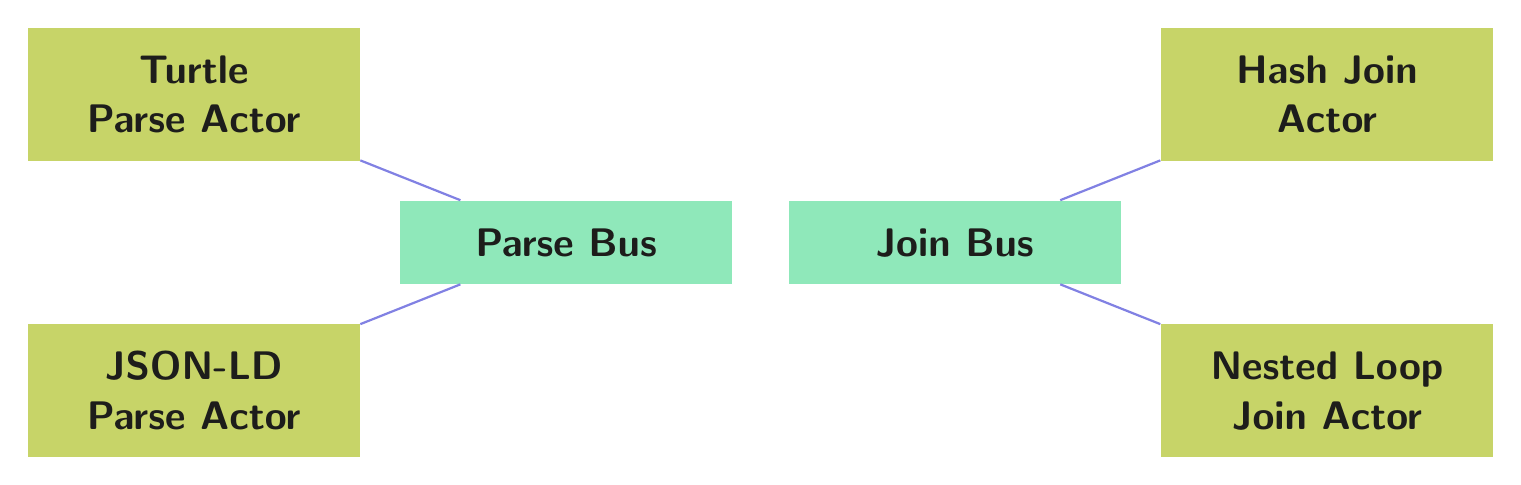
\begin{tikzpicture}[
    node distance = 2em, auto,
    font={\Large\itshape},
    base/.style={text=colortext,font={\Large\bfseries},inner sep=10pt,align=center,rectangle},
    txt/.style={text=colortext,font={},inner sep=7pt,align=center},
    action/.style={txt,color=coloraction},
    test/.style={txt,color=colortest},
    treenode/.style={base,thick,draw=colortext,text width=2em},
    relation/.style={text width=13em},
]

    \node[base,fill=colorbus,text width=10em]   (parsebus)       {Parse Bus};
    
    \node[base,fill=coloractor,text width=10em,above left=of parsebus] (actorparse1)    {Turtle Parse Actor};
    \node[base,fill=coloractor,text width=10em,below left=of parsebus] (actorparse2)    {JSON-LD Parse Actor};
    
    \draw[test,thick](parsebus) -- (actorparse1);
    \draw[test,thick](parsebus) -- (actorparse2);
    
    \node[base,fill=colorbus,text width=10em,right=of parsebus]   (joinbus)       {Join Bus};
    
    \node[base,fill=coloractor,text width=10em,above right=of joinbus] (actorjoin1)    {Hash Join Actor};
    \node[base,fill=coloractor,text width=10em,below right=of joinbus] (actorjoin2)    {Nested Loop Join Actor};
    
    \draw[test,thick](joinbus) -- (actorjoin1);
    \draw[test,thick](joinbus) -- (actorjoin2);

\end{tikzpicture}
\end{document}
